% http://users.ece.northwestern.edu/~sda690/MfB/Motion_CVPR08.pdf
% https://www.geeksforgeeks.org/opencv-motion-blur-in-python/
% https://www.wikiwand.com/en/Motion_blur
% http://tech.abdulfatir.com/2014/05/kernel-image-processing.html

+ Blur

\begin{figure}[H]
    \centering
    \begin{kmatrix}
    \matrix(img)[square matrix]{
        1 & 0 & 0 & 0 & 0 & 0 & 0 & 0 & 0 \\
        0 & 1 & 0 & 0 & 0 & 0 & 0 & 0 & 0 \\
        0 & 0 & 1 & 0 & 0 & 0 & 0 & 0 & 0 \\
        0 & 0 & 0 & 1 & 0 & 0 & 0 & 0 & 0 \\
        0 & 0 & 0 & 0 & 1 & 0 & 0 & 0 & 0 \\
        0 & 0 & 0 & 0 & 0 & 1 & 0 & 0 & 0 \\
        0 & 0 & 0 & 0 & 0 & 0 & 1 & 0 & 0 \\
        0 & 0 & 0 & 0 & 0 & 0 & 0 & 1 & 0 \\
        0 & 0 & 0 & 0 & 0 & 0 & 0 & 0 & 1 \\
    };

    \node[left=of img] {$\displaystyle\Scale[1.7]{\frac{1}{9}}$};
\end{kmatrix}

    \caption{Máscara de \textit{motion blur}: $h_9$.}
    \label{fig:h9}
\end{figure}

\begin{figure}[H]
    \centering
    \begin{subfigure}{0.48\textwidth}
        \centering
        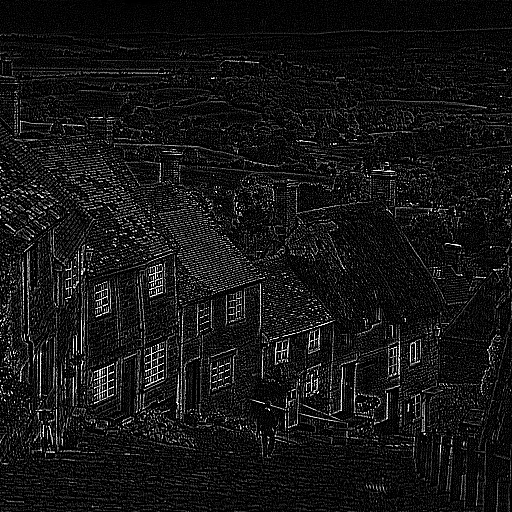
\includegraphics[width=0.9\textwidth]{imagens/city.png}
        \caption{Original: \texttt{city.png}.}
    \end{subfigure}%
    \begin{subfigure}{0.48\textwidth}
        \centering
        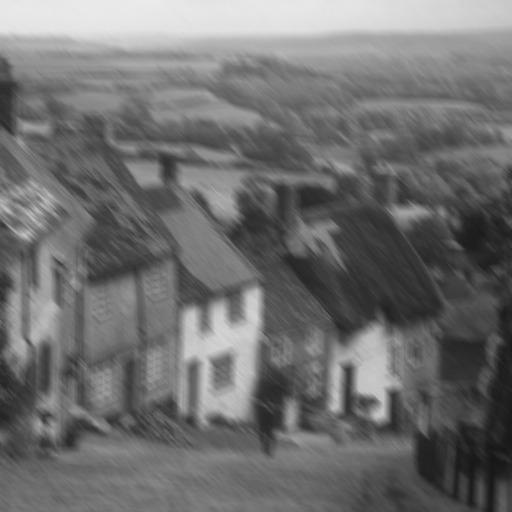
\includegraphics[width=0.9\textwidth]{resultados/city_h9.png}
        \caption{Convolução com $h_9$ (\ref{fig:h9}).}
    \end{subfigure}\\[8pt]
    \begin{subfigure}{0.48\textwidth}
        \centering
        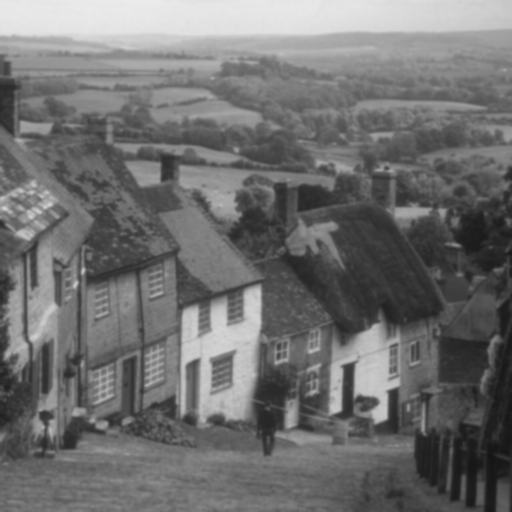
\includegraphics[width=0.9\textwidth]{resultados/city_h2.png}
        \caption{\textit{Blur} gaussiano (\hyperref[sec:blur]{$h_2$}).}
    \end{subfigure}

    \caption{Aplicação de \textit{motion blur}.}
    % \label{fig:blur}
\end{figure}
